\chapter{Determination of the grounding of the protocol}
\lhead{\emph{Appendices}} 
\label{app:grounding}	

The grounding of the communication is required when the protocol needs to be analysed. The determination of the grounding is done in 3 steps. In the first one, the interpretation given to each symbol of the vocabulary is determined. Then, the intent conveyed by each symbol is looked at. Finally, the information gained by the two preceding steps is merged to get the final grounding. Before looking at the grounding of the communication, the learned agents must be evaluated. Only protocol leading to an optimal solution are of interest. Afterwards, the greedy policy is determined by looking at the Q-estimate of each agent.

The following presents how the grounding is found. The example is taken from a training sessions with parameters $r_{com} = -0.1$, $r_{time} = -0.1$,  and $\gamma = 0.9$.

\paragraph*{Interpretations of the symbols}
The interpretation of the symbols by the feeding arms $agent_{arm1}$ and $agent_{arm2}$ is looked at first. In order to determine the interpretation, it is sufficient to look at what action the agent takes relative to the message received. Thus, only the states in which the agents could potentially transport a cube are of interest. If the agent decides to transport a cube, the message has been interpreted as "safe for me" and "not safe for me" otherwise. It is then possible to construct a table of interpretation and the right part of the protocol graph (tab.~\ref{tab:grounding-inter}, fig.~\ref{fig:grounding-inter}). 

\begin{table}[H]
\centering
\begin{minipage}[b]{.5\textwidth}
\vspace{0pt}
     \centering
    \begin{tabular}{lll}
    \toprule
    Symbol & $agent_{arm1}$ & $agent_{arm2}$ \\
    \midrule
    $v_0$ & not safe & not safe \\
    $v_1$ & not safe &  safe \\
    $v_2$ & not safe & not safe \\
    $v_3$ & safe & safe \\
    \bottomrule
    \end{tabular}
    \caption[Interpretation of symbols by the feeding agents]{Example of an interpretation of symbols by $agent_{arm1}$ and $agent_{arm2}$.}
    \label{tab:grounding-inter}
\end{minipage}%
\begin{minipage}[b]{.50\textwidth}
    \vspace{0pt}
    \centering
    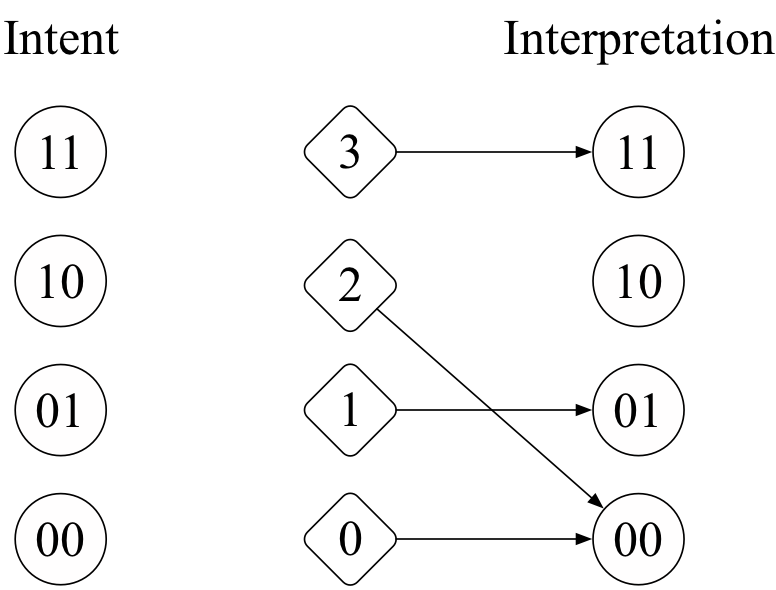
\includegraphics[width=0.75\textwidth]{imgs/grounding-inter.png}
    \caption[Protocol graph related to the interpretation of symbols by the feeding agents]{Protocol graph related to the interpretation of symbols by the feeding agents as shown in tab.~\ref{tab:grounding-inter}.}
    \label{fig:grounding-inter}
\end{minipage}
\end{table}

It is also possible to represent the assignment of the symbols using a set notation. This notation is useful when the grounding process needs to be implemented programmatically (tab.~\ref{tab:grounding-set-inter}).

\begin{table}[H]
\centering
\begin{minipage}[b]{.5\textwidth}
\vspace{0pt}
    \centering
    \begin{tabular}{lll}
    interpretation-$11$ & = & $\{v_3\}$ \\
    interpretation-$10$ & = & $\{\emptyset\}$ \\
    interpretation-$01$ & = & $\{v_1\}$\\
    interpretation-$00$ & = & $\{v_0, v_2\}$\\
    \end{tabular}
    \caption{Vocabulary assignment related to the interpretation.}
    \label{tab:grounding-set-inter}
\end{minipage}%
\begin{minipage}[b]{.50\textwidth}
    \vspace{0pt}
    \centering
    \begin{tabular}{lll}
    intent-$11$ & = & $\{v_1, v_3\}$ \\
    intent-$10$ & = & $\{v_2, v_0\}$ \\
    intent-$01$ & = & $\{v_1, v_2\}$\\
    intent-$00$ & = & $\{v_0, v_2\}$\\
    \end{tabular}
    \caption{Vocabulary assignment related to the intent.}
    \label{tab:grounding-set-intent}
\end{minipage}
\end{table}


\paragraph*{Intents of the symbols}
The intent transmitted by each symbol is then looked at. For this, the Q-table of $agent_{arm3c}$ is used. By looking at each sub state (see table~\ref{tab:agent3c-substate}), the sets containing the symbols relative to each intent can be constructed. Continuing with the same example, the sets presented in table~\ref{tab:grounding-set-intent} can be constructed. Based on this table, the protocol graph can then be completed (fig.~\ref{fig:grounding-intent}).

\begin{figure}[H]
    \vspace{0pt}
    \centering
    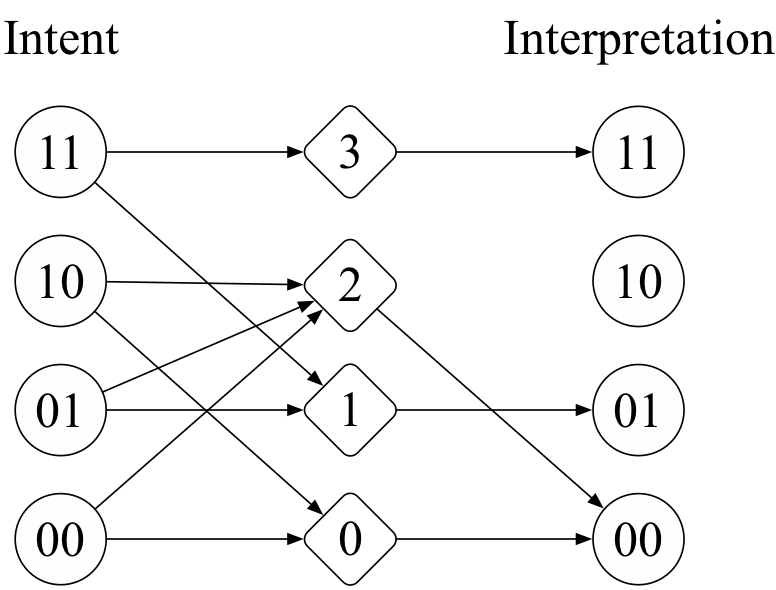
\includegraphics[width=0.375\textwidth]{imgs/grounding-intent.png}
    \caption[Protocol graph related to the intent of the symbols]{Protocol graph related to the intent transmitted by the symbols by the receiving agent.}
    \label{fig:grounding-intent}
\end{figure}

\paragraph*{Grounding of the protocol}

Finally, based on the sets in tables~\ref{tab:grounding-set-inter}~and~\ref{tab:grounding-set-intent}, it is possible to determine the final grounding of the communication. Table~\ref{tab:grounding-grounding} shows the final results for the example. The constructed sets enable the creation of the protocol graph depicting which intent is correctly transmitted through the channel (fig.~\ref{fig:grounding-final}).

\begin{table}[ht]
    \centering
    \begin{tabular}{lllll}
    grounding-$11$ & $=$ & intent-$11$ $\cap$ interpretation-$11$ & $= \{v_3\}$ \\ 
    grounding-$10$ & $=$ & intent-$10$ $\cap$ interpretation-$10$ & $= \{\emptyset\}$ \\ 
    grounding-$01$ & $=$ & intent-$01$ $\cap$ interpretation-$01$ & $= \{v_1\}$ \\ 
    grounding-$00$ & $=$ & intent-$00$ & $= \{v_0, v_2\}$ \\ 
    \end{tabular}
    \caption{Vocabulary assignment related to the grounding.}
    \label{tab:grounding-grounding}
\end{table}

\begin{figure}[H]
    \vspace{0pt}
    \centering
    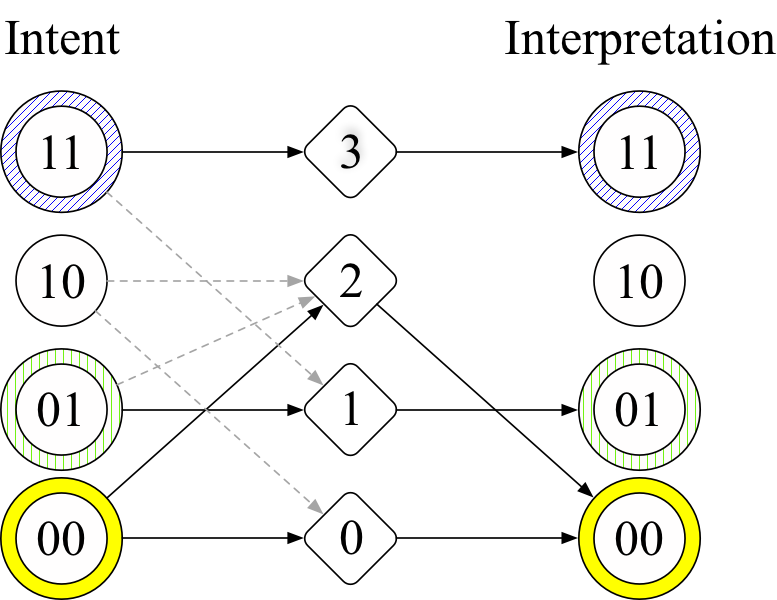
\includegraphics[width=0.375\textwidth]{imgs/grounding-final.png}
    \caption{Final protocol graph related to the example.}
    \label{fig:grounding-final}
\end{figure}

The protocol type of the example is thus $1011$. This learned protocol is non-ideal even though it leads to an optimal solution.
